
\section{Manifestation of Modbus protocol through Julia}
The objective of this experiment is to make the user acquainted with
the demonstration of Modbus protocol through the Julia-Arduino toolbox.
It gives an insight into how to acquire readings from the energy meter and interpret them accordingly. As explained in \secref{sec:energy-meter},
an energy meter is a device that gives us different electrical parameters, including voltage, current, and power, consumed by a device.
Here, we aim to obtain these values using the Julia-Arduino toolbox. For data transmission, we have used an RS485 module.

Julia is used for giving the required parameters to \arduino. For
example, the user will tell the required slave address to be accessed
and the number of registers to be read from or written to. Here,
\arduino\ acts as a master and energy meter as a slave. Therefore,
referring to a particular slave address will refer to the registers
that hold the desired electrical parameters (current, voltage, power, etc.), which we want to read from the energy meter.

In this experiment, \arduino\ is connected to the energy meter via an RS485 module which facilitates long-distance communication.
Julia sends the RQ to the \arduino\, which in turn sends it to the
energy meter. The energy meter then accesses the values in the
required addresses in its memory and transfers them back. This again
is in the form of another packet called RP. In this packet, the data is stored in a little-endian hexadecimal format. Thus, we make use of IEEE 754 to obtain the decimal value from this data.

\paragraph{Note: } The Julia source files presented in this section were tested on the older versions. Now, these codes may require minor changes in
the newer versions. We invite the experts to contribute the revised version of the code.


% \subsection{Software for the experiment}
% Apart from the Julia-Arduino toolbox, the software for this experiment comprises two parts:
% \begin{enumerate}
% \item  Firmware for \arduino: This firmware is needed to communicate
% with Julia (using serial interface), and with RS485 module (using
% Software Serial interface). Control logic to enable receive and
% transmit modes of MAX485 chip is also present in this firmware. \figref{fig:modbus-firmware} demonstrates the overall implementation of this firmware.

% \begin{figure}
%   \centering
%   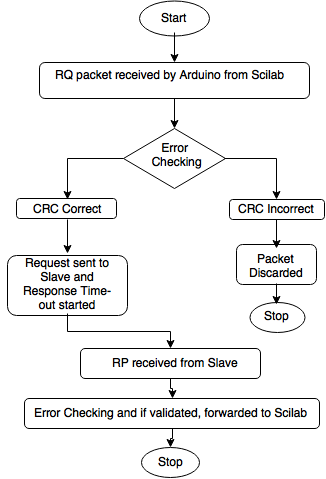
\includegraphics[width=\lgfig]{\LocMODfig/arduino_code_flowchart.png}
%   \caption{Flowchart of Arduino firmware}
%   \label{fig:modbus-firmware}
% \end{figure}

% \item Julia source file: It requests the parameters in the energy meter
% by sending an RQ to \arduino\ from Julia. Then it waits till
% an RP is available from the \arduino. After receiving the RP, it extracts 
% the data from this packet and converts it into IEEE
% 754 floating-point format. The overall implementation is being
% described below:
% \begin {enumerate}
% \item Frame an RQ to be sent to the energy meter (slave) in ASCII coded decimal
% format. 
% \item Send the RQ serially to \arduino. 
% \item Let \arduino\ send the RQ to the energy meter via RS485 module. 
% \item Let the energy meter send the RP to \arduino\ via RS485 module. 
% \item Read the RP available on \arduino. 
% \item Extract the data stored in holding registers from the RP. 
% \item Assuming this data to be stored in little-endian format, 
% convert this data in floating-point values using IEEE 754 standard. 
% \item Display the value in the Command Prompt (on Windows) or Terminal (on Linux), as the case maybe. 
% \end{enumerate}
% \figref{fig:flow-chart} presents the sequence in which the steps mentioned above are executed. 
% \begin{figure}
%   \centering
%   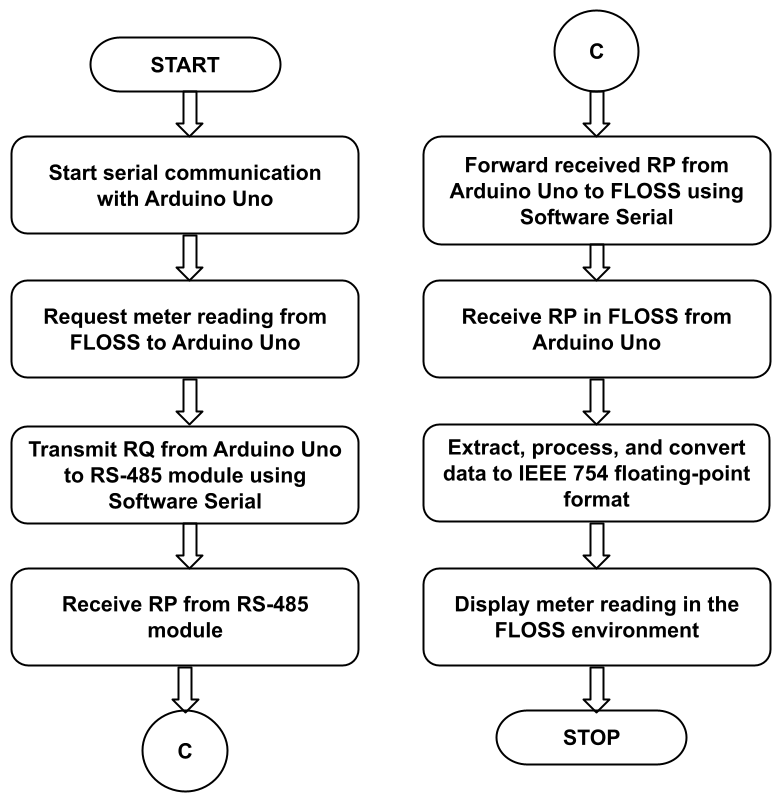
\includegraphics[width=\hgfig]{\LocMODfig/flowchart.png}
%   \caption{Flowchart of the steps happening in Julia code}
%   \label{fig:flow-chart}
% \end{figure}
% \end{enumerate}


\section{Reading the electrical parameters from Julia}
\subsection{Reading the electrical parameters}
In this section, we will show how to access the three parameters (voltage, current, and active power) in the energy meter. As discussed above, we will send an RQ from Julia to \arduino. Subsequently, \arduino\ will provide us with an RP, which can be decoded to extract the desired parameter. The reader should go through the instructions given in \secref{sec:julia-start} before getting started.

\subsection{Julia Code}
\label{sec:modbus-julia-code}
\addtocontents{juliad}{\protect\addvspace{\codclr}}

\begin{juliacode}
  \jcaption{Code for Single Phase Current Output}
  {Code for Single Phase Current Output.
    Available at \LocMODjuliabrief{readCurrent.jl}.}
  \label{julia:current-modbus}
  \lstinputlisting[firstline=1,lastline=10]
  {\LocMODjuliacode/readCurrent.jl}
\end{juliacode}

\begin{juliacode}
  \jcaption{Code for Single Phase Voltage Output}
  {Code for Single Phase Voltage Output.
    Available at \LocMODjuliabrief{readVoltage.jl}.}
  \label{julia:voltage-modbus}
  \lstinputlisting[firstline=1,lastline=10]
  {\LocMODjuliacode/readVoltage.jl}
\end{juliacode}

\begin{juliacode}
  \jcaption{First 10 lines of the code for Single Phase Active Power
    Output}{First 10 lines of the code for Single Phase Active Power
    Output.  Available at
    \LocMODjuliabrief{readPower.jl}.}
  \label{julia:modbus-power}
  \lstinputlisting[firstline=1,lastline=10]
  {\LocMODjuliacode/readPower.jl}
\end{juliacode}
